%!TEX root = ../../dissertation.tex
%%%%%%%%%%%%%%%%%%%%%%%%%%%%%%%%%%%%%%%%%%%%%%%%%%%%%%%%%%%%%%%%%%%%%%%%%%%%%%%%
\section{Evaluation Methodology}
\label{c4:methodology}

With the mobile network load defined and possible influencing factors described, we now move on to apply these to an actual mobile network. For this data from passive network traces will be employed. But first, the monitoring setup and the captured has to be described in this section. This also includes a description of some methods required to examine specific device types and other device-based factors from the dataset.

While this chapter only employs passive measaurements, Chapter~\ref{chap:mobilestreaming} will additionaly deal with approaches to conduct meaningful active device-based measurements and additionally set up a simulation/emulation testbed based on the results.

%%%%%%%%%%%%%%%%%%%%%%%%%%%%%%%%%%%%%%%%%%%%%%%%%%%%%%%%%%%%%%%%%%%%%%%%%%%%%%%%
\subsection{Network and Monitoring Setup}

For our analysis, the \gls{METAWIN} monitoring system developed in a previous third-party research project and deployed in the network of an Austrian mobile operator is used. \cite{ricciato_2011,ricciato2006traffic}

\begin{figure}[htb]
	\centering
	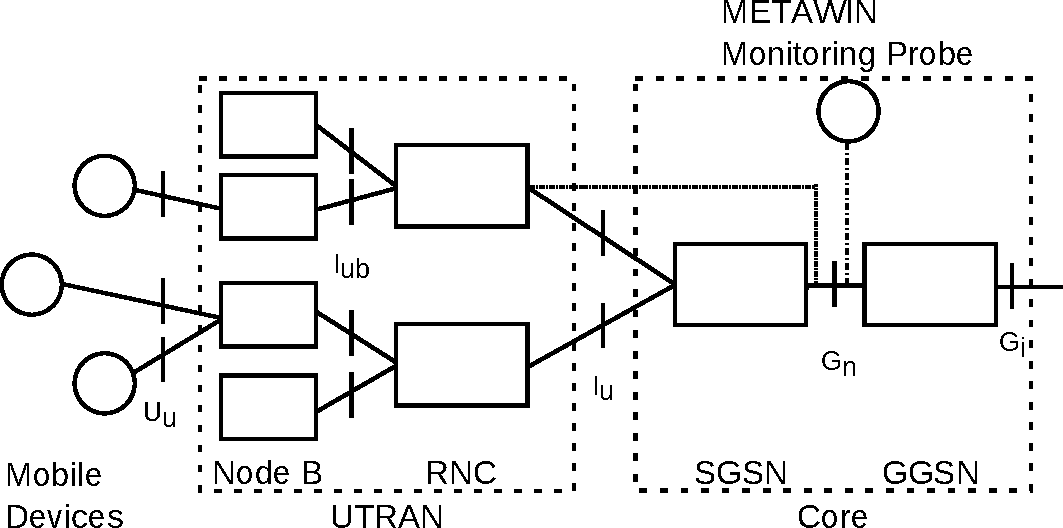
\includegraphics[width=1.0\textwidth]{images/umts-network.pdf}
	\caption{Location of the \acrshort{METAWIN} monitoring probe in the \gls{3G} core network}
	\label{c4:fig:umtsnetwork}
\end{figure}


The measurement taps are located at the Gn interface at one \gls{GGSN} within the core network as depicted in Figure~\ref{c4:fig:umtsnetwork}. It gives access to a wide spectrum of core \gls{gtp} signaling, including the mobility and tunnel management. \cite{3gpp.29.060}. The system does not offer a complete packet trace, but aggregates every signaling transaction and user traffic flow down to a number of select fields. This includes \gls{gtp} \gls{IE} such as the \gls{RAT}  as well as the terminal types of the mobile clients. The latter is determinable by the \gls{TAC} part of the \gls{IMEI} (cf.~\cite{3gpp.23.003}) and will be discussed later in detail.

In the network under study, a direct tunnel setup might be used for \gls{UMTS}-using \glspl{UE} consisting of a direct link between \glspl{GGSN} and the \glspl{RNC} and circumventing the \gls{SGSN}. It is only used for transporting user-plane traffic, signaling procedures are carried out in the normal way between \glspl{SGSN} and \gls{GGSN}. Therefore, only the Gn interface at \gls{GGSN} is seeing the complete core network traffic, explaining the location of the tap. The network under study has more than one \gls{GGSN} at different physical locations. The tapped \gls{GGSN} manages about half of the operator's total traffic volume in this period. 

Recording data in a live network necessitates meeting strict privacy requirements regarding the handling of user-related data. \gls{METAWIN} complies with this by anonymizing all user-identifying. Application-level payload is removed and all user identifiers (e.g. \gls{IMSI}) are non-reversibly hashed before recording. \glspl{UE} in a dataset can still be differentiated by the hashes but not traced back to the actual user. The wiretaps deployed within the monitoring system are time-synchronized with \gls{GPS}. Accordingly, the packet timestamps have an accuracy of least \SI{100}{\nano\second}.
%~\cite[p.97-98]{donnelly_high_2002}.


%%%%%%%%%%%%%%%%%%%%%%%%%%%%%%%%%%%%%%%%%%%%%%%%%%%%%%%%%%%%%%%%%%%%%%%%%%%%%%%%
\subsection{Dataset Description}

Using \gls{METAWIN} a week-long core trace was acquired. It was recorded in April 2011, specifically begining at Monday, \yyyymmdddate\formatdate{10}{4}{2011}, \formattime{0}{0}{0} and ending Sunday, \formatdate{17}{4}{2011}, \formattime{23}{59}{59}.

The trace includes user plane as well as control plane traffic. User plane traffic is recorded in a traffic flow granularity with the trace containing data on \num{2.2e9} aggregated flows. No exact flow start time is given, instead it is rounded down to a \SI{2}{\hour} window with the timestamp at the beginning. A flow entry further consists of hashed identifiers for the gls{IMSI} and the remote server. Besides the usual protocol and port information, the transmitted data volume, in a number of packet as well as byte count, is given on in both link directions. Additional information is available on \gls{HTTP} traffic. This portion of the trace includes precise timestamps as well as the \acrshort{MIME}-type, result code, and size of the requested objected.

The recorded control plane traffic consists of \num{4.1e8} \gls{gtp} tunnel management transactions, i.e. every create, update, and delete request and response. Not all of the \glspl{IE} data is included. But most importantly, it includes the \gls{TAC}, \gls{RAT} and hashed \gls{IMSI} for the purpose of device discrimination. Also present are several timestamps with \SI{64}{\bit} precision describing the time of the request, response and the tunnel's start time. Finally, the \gls{gtp} data contains the response codes for each request. With these codes, failed transactions can be distinguished from successful ones and examined separately. Since the hashed \gls{IMEI} is consistent across the user and control plane data, both can be cross-correlated.

All trace information was exported from \gls{METAWIN} as pure line-based text data. For this investigation all records were fed into a \acrshort{SQL} database. Evaluations were conducted through scripted queries on the database.  

%%%%%%%%%%%%%%%%%%%%%%%%%%%%%%%%%%%%%%%%%%%%%%%%%%%%%%%%%%%%%%%%%%%%%%%%%%%%%%%
\subsection{Device Identification}

Individual device types can also be identified in the data througth the \gls{TAC} field on every entry.The \gls{TAC} represents the first eight decimal digits of the \gls{IMEI} and uniquely identifies each device type \cite{3gpp.23.003}. The following six digits of the \gls{IMEI} constitute the serial number of a specific device, which is of course omitted in the data. Due to the short length of this serial number, popular devices will often be assigned more than one \gls{TAC}, somewhat complicating the identification of certain device models.

\glspl{TAC} are assigned to individual device models by the regional members, or \gls{RBI}, of the \gls{GSMA}, distinguished by the first two digits of the \gls{TAC}. The full allocation information is not freely available, but only to members of the \gls{GSMA}, which is not a viable option for research institutions and other interested parties. Some independent efforts have been made to collect \glspl{TAC} from devices. Most of them allow just low-volume queries for specific \glspl{TAC} for non-commercial purposes. However, one \gls{TAC} dataset is publicly available and can be used freely. \footnote{Available at \url{http://www.mulliner.org/tacdb/}.}

This evaluation is based uses this dataset, with some additional device identifiers collected during the course of the investigation. With this at hand, many of the devices associated with the flows and \gls{gtp} messages from the trace were iteratively identified and categorized.
% we went through large portions of the \glspl{TAC} present in our dataset, and identified and categorized the most important entries. In this case, importance means various metrics like the traffic volume, the number of flows, and the number of \gls{gtp} signaling messages for each \gls{TAC}. 



%%%%%%%%%%%%%%%%%%%%%%%%%%%%%%%%%%%%%%%%%%%%%%%%%%%%%%%%%%%%%%%%%%%%%%%%%%%%%%%%
\subsection{\texorpdfstring{\acrshort{TAC}}{TAC} Evaluation Validity}

It is important to know whether the information available in the \gls{TAC} dataset covers enough of the devices seen in the traces to conduct sufficiently meaningful evaluations. After all, the \gls{TAC} data is large albeit still very incomplete due to the sheer number of devices in existence.

\begin{table}
\centering
\caption{Relative \acrshort{TAC} Statistics.}
\label{c4:tbl:tacstats}
	\begin{tabu}{XX[r]}
		\toprule
		\textbf{Type} & \textbf{Portion of devices with entry in TAC DB}\\ 
		\midrule
		Total number of flows & $99.72\%$ \\
		Ratio of total traffic & $99.97\%$\\
		Total number of tunnels & $87.57\%$ \\
		Total number of \gls{gtp} signaling messages & $90.95\%$ \\
		Number of distinct \glspl{UE} & $80.93\%$\\ 
		\bottomrule
	\end{tabu}
\end{table}

Table~\ref{c4:tbl:tacstats} provides statistics on identified knowledge of devices in the dataset. About $80\%$ of all distinct devices active could be identified. Looking at the total number of \gls{gtp} signaling messages, we see that we can determine the device name of over $90\%$.
The flow data shows an even clearer picture, as we can identify almost all of the devices involved.



As we are working with an incomplete \gls{TAC} database it is important to know whether our \gls{TAC} mappings provide sufficiently useful data to allow for the envisioned device discriminating statistics. Therefore, Table~\ref{c4:tbl:tacstats} provides some statistics on our knowledge of devices in the dataset. About 80 percent of all distinct and active devices could be identified. Looking at the total number of \gls{gtp} signaling messages, we see that we can determine the device name of over 90 percent. The flow data shows an even clearer picture, as we can identify almost all of the devices involved.



%%%%%%%%%%%%%%%%%%%%%%%%%%%%%%%%%%%%%%%%%%%%%%%%%%%%%%%%%%%%%%%%%%%%%%%%%%%%%%%%
\subsection{Device Classification}

For our investigation, we went through large portions of the \glspl{TAC} present in our dataset, and identified and categorized the most important entries. In this case, importance means various metrics like the traffic volume, the number of flows, and the number of \gls{gtp} signaling messages for each \gls{TAC}. 


After having available the device names for most \glspl{TAC}, we were able to add meta-information and categorize the entries based on their device type and operating system. For the device type we partitioned the devices roughly into smartphones, regular mobile phones and 3G USB dongles or 3G/WiFi routers. The operating system includes most of the popular incarnations found in the network at measurement time, including Android, iOS, and Symbian. Note however that many devices, especially USB dongles cannot be linked to any specific OS.


After having available the device names for most \glspl{TAC}, we were able to add meta-information to the entries in form of the following categories:

\begin{itemize}
\item The device type. We distinguished between smartphones, regular mobile phones and feature phones, and 3G USB dongles or 3G/WiFi routers.

\item The operating system of the device (if known), such as Android, iOS, Series 40, BlackBerry OS etc. This is especially interesting to identify potential differences in the core network signaling patterns of devices. Note however that we cannot link USB dongles and OS types from the \gls{TAC}.

\end{itemize}

\todo{extend this section}


%%%%%%%%%%%%%%%%%%%%%%%%%%%%%%%%%%%%%%%%%%%%%%%%%%%%%%%%%%%%%%%%%%%%%%%%%%%%%%%%
\subsection{Preliminary Device Statistics}
After applying the categorization to the \glspl{TAC} we evaluate the device composition in the network. The two largest portions of devices are smartphones  and 3G dongles, while classic cell phones do not seem to play a major role anymore. 
%We see about twice as many Android as iOS devices, possibly attributed either to the contractual situation of the operator or the wider price range of Android devices.

%Regular phones have negligible user traffic despite still making up one tenth of the device fraction. 


Initially, one planned endeavor was to investigate possible peculiarities of business phone behavior, especially of those easily identifiable Blackberry OS phones, but the number of distinct Blackberry devices in the dataset is too low to draw conclusions of any significance.

One observation across all device types is that about 18 percent of all mobile devices have activated their mobile data service and have signaling traffic, but do not cause any use plane traffic.

The difference between 3G dongles and smartphones is also noteworthy. While the former cause large amounts of user plane traffic (compared to the device numbers), they are responsible for but a low number of core network signaling events and tunnels. This picture is reversed for smartphones.

After applying the categorization to the \glspl{TAC} we evaluate the device composition in the network. The two largest portions of devices are smartphones and 3G dongles, while classic cell phones do not seem to play a major role in the packet-switched domain anymore. One observation across all device types is that about 14 percent of all mobile devices have activated their mobile data service and have signaling traffic, but do not cause any user plane traffic.

The difference between 3G dongles and smartphones is also noteworthy. While the former cause large amounts of user plane traffic (compared to the device numbers), they are responsible for but a few core network signaling events and tunnels. This picture is reversed for smartphones.





